\documentclass[a4paper]{article}
\usepackage[]{graphicx}\usepackage[]{color}
% maxwidth is the original width if it is less than linewidth
% otherwise use linewidth (to make sure the graphics do not exceed the margin)
\makeatletter
\def\maxwidth{ %
  \ifdim\Gin@nat@width>\linewidth
    \linewidth
  \else
    \Gin@nat@width
  \fi
}
\makeatother

\definecolor{fgcolor}{rgb}{0.345, 0.345, 0.345}
\newcommand{\hlnum}[1]{\textcolor[rgb]{0.686,0.059,0.569}{#1}}%
\newcommand{\hlstr}[1]{\textcolor[rgb]{0.192,0.494,0.8}{#1}}%
\newcommand{\hlcom}[1]{\textcolor[rgb]{0.678,0.584,0.686}{\textit{#1}}}%
\newcommand{\hlopt}[1]{\textcolor[rgb]{0,0,0}{#1}}%
\newcommand{\hlstd}[1]{\textcolor[rgb]{0.345,0.345,0.345}{#1}}%
\newcommand{\hlkwa}[1]{\textcolor[rgb]{0.161,0.373,0.58}{\textbf{#1}}}%
\newcommand{\hlkwb}[1]{\textcolor[rgb]{0.69,0.353,0.396}{#1}}%
\newcommand{\hlkwc}[1]{\textcolor[rgb]{0.333,0.667,0.333}{#1}}%
\newcommand{\hlkwd}[1]{\textcolor[rgb]{0.737,0.353,0.396}{\textbf{#1}}}%
\let\hlipl\hlkwb

\usepackage{framed}
\makeatletter
\newenvironment{kframe}{%
 \def\at@end@of@kframe{}%
 \ifinner\ifhmode%
  \def\at@end@of@kframe{\end{minipage}}%
  \begin{minipage}{\columnwidth}%
 \fi\fi%
 \def\FrameCommand##1{\hskip\@totalleftmargin \hskip-\fboxsep
 \colorbox{shadecolor}{##1}\hskip-\fboxsep
     % There is no \\@totalrightmargin, so:
     \hskip-\linewidth \hskip-\@totalleftmargin \hskip\columnwidth}%
 \MakeFramed {\advance\hsize-\width
   \@totalleftmargin\z@ \linewidth\hsize
   \@setminipage}}%
 {\par\unskip\endMakeFramed%
 \at@end@of@kframe}
\makeatother

\definecolor{shadecolor}{rgb}{.97, .97, .97}
\definecolor{messagecolor}{rgb}{0, 0, 0}
\definecolor{warningcolor}{rgb}{1, 0, 1}
\definecolor{errorcolor}{rgb}{1, 0, 0}
\newenvironment{knitrout}{}{} % an empty environment to be redefined in TeX

\usepackage{alltt}
\newcommand{\SweaveOpts}[1]{}  % do not interfere with LaTeX
\newcommand{\SweaveInput}[1]{} % because they are not real TeX commands
\newcommand{\Sexpr}[1]{}       % will only be parsed by R



\usepackage[utf8]{inputenc}
\pagenumbering{arabic}
%\usepackage[ngerman]{babel}
\usepackage{a4wide,paralist}
\usepackage{amsmath, amssymb, xfrac, amsthm}
\usepackage{dsfont}
\usepackage[usenames,dvipsnames]{xcolor}
\usepackage{amsfonts}
\usepackage{graphicx}
\usepackage{caption}
\usepackage{subcaption}
\usepackage{framed}
\usepackage{multirow}
\usepackage{bytefield}
\usepackage{csquotes}
\usepackage[breakable, theorems, skins]{tcolorbox}
\usepackage{hyperref}
\usepackage{cancel}
\usepackage{bm}

\input{../../style/common}

\tcbset{enhanced}

%exercise numbering
\renewcommand{\theenumi}{(\alph{enumi})}
\renewcommand{\theenumii}{\roman{enumii}}
\renewcommand\labelenumi{\theenumi}

\font \sfbold=cmssbx10
\setlength{\oddsidemargin}{0cm} \setlength{\textwidth}{16cm}

\sloppy
\parindent0em
\parskip0.5em
\topmargin-2.3 cm
\textheight25cm
\textwidth17.5cm
\oddsidemargin-0.8cm
% \pagestyle{empty}

\newcommand{\kopf}[1] {
\hrule
\vspace{.15cm}
\begin{minipage}{\textwidth}
	{\sf \bf \huge Exercise Collection -- #1}
\end{minipage}
\vspace{.05cm}
\hrule
\vspace{1cm}}

\newcommand{\exlect}
  {\color{black} \hrule \section{Lecture exercises}}
  
\newcommand{\exexams}
  {\color{black} \hrule \section{Questions from past exams}}
  
\newcommand{\exinspo}
  {\color{black} \hrule \section{Ideas \& exercises from other sources}}

\newcounter{aufg}
\newenvironment{aufgabe}[1]
	{\color{black} \refstepcounter{aufg}
	\subsection{Exercise \arabic{aufg}: #1} 
	\noindent}
	{\vspace{0.5cm}}
	
\newenvironment{aufgabeexam}[3] % semester, main or retry exam, question number
	{\color{black} \refstepcounter{aufg}
	\subsection{Exercise \arabic{aufg}: #1, #2 exam, question #3}
	\noindent}
	{\vspace{1.5cm}}

\newcounter{loes}
\newenvironment{loesung}
	{\color{gray} \refstepcounter{loes}\textbf{Solution \arabic{loes}:}
	\\ \noindent}
	{\bigskip}

\setcounter{secnumdepth}{0}



\begin{document}
% !Rnw weave = knitr



\input{../../latex-math/basic-math.tex}
\input{../../latex-math/basic-ml.tex}

\kopf{Supervised Classification}

\tableofcontents

% ------------------------------------------------------------------------------
% LECTURE EXERCISES
% ------------------------------------------------------------------------------

\dlz
\exlect
\lz

\aufgabe{logistic regression -- thresholding}{

In logistic regression, we estimate the probability $\pix = \post$.
To decide if $\hat{y}$ is $0$ or $1$, we follow:

$$
\hat{y} = 1 \ \ \Leftrightarrow \ \ \pixh \geq a
$$


\begin{itemize}
\item[a)] What happens if you are choosing $a = 0.5$? More precisely, from which value of $\thetab^T \xv$ do you predict $\hat{y} = 1$ rather than $\hat{y} = 0$?
\item[b)] Explain (using words) why $a = 0.5$ is a sensible threshold.
\end{itemize}
}

\newpage
\loesung{

\begin{enumerate}
\item %Logistic regression is a classification model, that estimates posterior probabilities $\pi(x)$ by linear functions in $x$.
For a binary classification problem the model can be written as:\\

$$
\hat{y} = 1 \ \ \Leftrightarrow \ \ \pix = \frac{1}{1 + \exp(-\thetab^T \xv)} \geq a
$$

This can be reformulated, s.t. for $a \in (0,1)$

\begin{align*}
&\frac{1}{1 + \exp(-\thetab^T \xv)} \geq a \\
\Leftrightarrow\ & 1 + \exp(-\thetab^T \xv) \leq a^{-1} \\
\Leftrightarrow\ & \exp(-\thetab^T \xv) \leq a^{-1} - 1 \\
\Leftrightarrow\ & -\thetab^T \xv \leq \log(a^{-1} - 1) \\
\Leftrightarrow\ & \thetab^T \xv \geq -\log(a^{-1} - 1) \\
\end{align*}



For $a = 0.5$ we get:

$$
\hat{y} = 1 \ \ \Leftrightarrow \ \ \thetab^T \xv \geq -\log(0.5^{-1} - 1) = -\log(2 - 1) = -\log(1) = 0
$$
This means the linear decision boundary is defined by a hyperplane equation, i.e.,  
$\thetab^T \xv = 0$
and it divides the input space in the "1"-space ($\thetab^T \xv \geq 0$) and in the "0"-space ($\thetab^T \xv < 0$).
\item  When the threshold $a = 0.5$ is chosen, the losses of missclassified observations, i.e., $L(\hat{y}=0|y=1)$ and  $L(\hat{y}=1|y=0)$ ,  are weighted equally. This means $a = 0.5$ is a sensible threshold if one does not need to avoid one type of misclassification more than the other.\\
Intuitively it makes sense to cut off at $0.5$ because, if the probability for 1 is closer to 1 than to 0, we would intuitively choose 1 rather than 0.
\end{enumerate}
}

\aufgabe{logistic regression -- link function and likelihood}{

\begin{enumerate}
  \item[a)] What is the relationship between softmax $\pi_k(x)=\frac{\exp(\theta_k^T x)}{\sum^g_{j=1} \exp(\theta_j^T x)}$ and the logistic function $\pix =\frac{1}{1+\exp(-\theta^{T} x)}$ for $g = 2$ (binary classification)?

  \item[b)] The likelihood function of a multinomially distributed target variable with $g$ target classes is given by
 $$\mathcal{L}_i = \P(Y^{(i)} = y^{(i)}|x^{(i)},\theta_1, \dots, \theta_g) = 
\prod^g_{j=1} \pi_j(x^{(i)})^{\mathds{1}_{\{y^{(i)} = j\}}}$$
where the posterior class probablities $\pi_1(x), \dots, \pi_g(x)$ are modeled with softmax regression.
  Derive the likelihood function of $n$ such independent target variables. How can you transform this likelihood function into an empirical risk function?
  \\ Hints: 
  \begin{itemize}
  \item By following the maximum likelihood principle, we should look for parameters $\theta_1, \dots, \theta_g$, which maximize the likelihood function.
  \item The expressions $\prod \mathcal{L}_i$ and $\log\prod\mathcal{L}_i$ (if this expression is defined) are maximized by the same parameters.
  \item The empirical risk is a \emph{sum} of loss function values, not a \emph{product}.
  \item Minimizing a scalar function multiplied with -1 is equivalent to maximizing the original function.
  \end{itemize}
  State the associated loss function. 

  \item[c)] Explain how the predictions of softmax regression (multiclass classification) look like (probabilities and classes) and define the parameter space.

  % \item[c)] Calculate the derivative of the negative likelihood as a loss function for softmax regression: $\triangledown_{\theta_k}L= \sum_{i=1}^n {-x ([y[i]==k] - \pi_k)}$ (suppose there are n instances)
\end{enumerate}

}
\newpage
\loesung{

\begin{enumerate}

  \item[a)]

  $\pi_1(x)=\frac{\exp(\theta_1^T x)}{\exp(\theta_1^T x) + \exp(\theta_2^T x)}$

  $\pi_2(x)=\frac{\exp(\theta_2^T x)}{\exp(\theta_1^T x) + \exp(\theta_2^T x)}$

  $\pi_1(x)=\frac{1}{ (\exp(\theta_1^T x) + \exp(\theta_2^T x) )/ \exp(\theta_1^T x)} = \frac{1}{1+\exp(-\theta^{T} x)}$ where $\theta =\theta_1 - \theta_2 $ and $\pi_2(x) = 1 - \pi_1(x)$

  \item[b)]
  When using softmax regression the posterior class probability for the class $k$ is modeled, s.t.
  $$\pi_k(x) = \frac{\exp(\theta_k^T x)}{\sum^g_{j=1} \exp(\theta_j^T x)}.$$ 
  
  A single observation is multinomially distributed, i.e., 
$$\mathcal{L}_i = \P(Y^{(i)} = y^{(i)}|x^{(i)},\theta_1, \dots, \theta_g) = 
\prod^g_{j=1} \pi_j(x^{(i)})^{\mathds{1}_{\{y^{(i)} = j\}}}.$$
  Under the assumption that the observations are conditionally independent the 
  likelihood of the data can be expressed, s.t.
  $$\mathcal{L} = \P(Y^{(1)} = y^{(1)},\dots,Y^{(n)} = y^{(n)}|x^{(1)},\dots,x^{(n)},\theta_1, \dots, \theta_g) = \prod^n_{i=1}\prod^g_{j=1} \pi_j(x^{(i)})^{\mathds{1}_{\{y^{(i)} = j\}}}.$$
(By following the maximum likelihood principle, we should look for parameters $\theta_1, \dots, \theta_g$, which maximize the expression above.) \\
 Now we want the empirical risk to be a \emph{sum} of loss function values, not a \emph{product}
recall: $$\riske = \sum^n_{i=1} \Lxyi.$$
We can turn the product into a sum by taking its log since the same parameters maximize the expressions. Finally, we convert the maximization into minimization by multiplying with -1. So we end up with the so-called cross-entropy loss function:
  
$$ \Lxy = -\sum^g_{j=1} \mathds{1}_{\{y = j\}}\log[{\pi_j(x)}].$$
 
We see that for the softmax regression the loss function is equal to the negative log-likelihood of one observation. Thus the associated empirical risk is the negative log-likelihood of the complete data set.
  
  \item[c)]
  Since the subtraction of any fixed vector from all $\theta_k$ does not change the prediction, one set of parameters is "redundant". Thus we set $\theta_g = (0,\dots,0).$
    Hence for $g$ classes we get $g - 1$ discriminant functions from the softmax $\hat{\pi}_1(x), \dots, \hat{\pi}_{g-1}(x)$ which can be interpreted as probability. The probability for class $g$ can be calculated by using $\hat{\pi}_g = 1 - \sum_{k = 1}^{g-1} \hat{\pi}_k(x)$. To estimate the class we are using majority vote:
    $$
    \hat{y} = \argmax_k \hat{\pi}_k(x)
    $$
    The parameter of the softmax regression is defined as parameter matrix where each class has its own parameter vector $\theta_k$, $k \in \{1, \dots, g-1\}$:
    $$
    \theta = [\theta_1, \dots, \theta_{g-1}]
    $$



  % $\frac{\partial (-\log L)}{\partial \theta_i} = - \sum_k I_k \frac{1}{\pi_k} \frac{\partial \pi_k}{\partial \theta_i}$

  % since

  % $ \frac{\partial \pi_i}{\partial \theta_i} = \triangledown_{\theta_i} \frac{e^{\theta_i^T x}}{\sum_k e^{\theta_k^T x}}= \frac{e^{z_i}(\sum_k e^{z_k})-(e^{z_i})^2}{(\sum_k e^{z_k})^2}x = \frac{e^{z_i}(\sum_{k \neq i} e^{z_k})}{(\sum_k e^{z_k})^2}x= \pi_i(1 - \pi_i)x$,

  % $ \frac{\partial \pi_i}{\partial \theta_j} = \triangledown_{\theta_j} \frac{e^{\theta_i^T x}}{\sum_k e^{\theta_k^T x}}= \frac{-e^{z_i}e^{z_j}}{(\sum_k e^{z_k})^2}x= - \pi_i\pi_j x$, ($i \neq j$)

  % Conclusion:

  % $\frac{- \partial \log L}{\partial \theta_i} = - \sum_k I_k \frac{1}{\pi_k} \frac{\partial \pi_k}{\partial \theta_i} = -(1-\pi_i)x$ ($i = y$)
  % and

  % $\frac{- \partial \log L}{\partial \theta_j} = - \sum_k I_k \frac{1}{\pi_k} \frac{\partial \pi_k}{\partial \theta_j} = \pi_j x$
  % ($j \neq y$)

  % Writing the two cases in one formula, we have

  % $\frac{- \partial \log L}{\partial \theta_k} = -(I_k -\pi_k )x$ where $I_k = [y = k]$

  % summing over all instances, we have

  % $\triangledown_{\theta_k}\mathcal{L} = \sum_{i=1}^n-([y_i = k] -\pi_k )x$
\end{enumerate}

}

\aufgabe{logistic regression -- softmax hyperplane}{

Summarize the logistic regression model (shortly!). Show that the decision boundaries, which are defined as the area where the estimated probability for class 1 is exactly a specific threshold $a \in [0, 1]$, is always a hyperplane between both classes. What happens if you are choosing $a = 0.5$?
}
\dlz
\loesung{

Logistic regression is a classification model, that estimates posterior probabilities $\pi(x)$ by linear functions in $x$.
For a binary classification problem the model can be written as:\\

$$
\hat{y} = 1 \ \ \Leftrightarrow \ \ \pi(x) = \frac{1}{1 + \exp(-x^T\theta)} \geq a
$$

For the decision boundary we have to set $\pi(x) = a$. Solving this equation for $x$ yields:

\begin{align*}
&\frac{1}{1 + \exp(-x^T\theta)} = a \\
\Leftrightarrow\ & 1 + \exp(-x^T\theta) = a^{-1} \\
\Leftrightarrow\ & \exp(-x^T\theta) = a^{-1} - 1 \\
\Leftrightarrow\ & \exp(-x^T\theta) = a^{-1} - 1 \\
\Leftrightarrow\ & -x^T \theta = \log(a^{-1} - 1) \\
\Rightarrow\ & x^T \theta = -\log(a^{-1} - 1) \\
\end{align*}

For $a = 0.5$ we get:

$$
x^T \theta = -\log(0.5^{-1} - 1) = -\log(2 - 1) = -\log(1) = 0
$$

% $$
% \log\frac{\P(y = 1 | x)}{\P(y = 0 | x)} = \beta^T x
% $$
% We want to model the probability for class 1:
% $$
% \P(y = 1 | x) = \frac{\exp(\beta^T x)}{1 + \exp(\beta^T x)} = \frac{\exp(f(x))}{1 + \exp(f(x))}
% $$
% Let $\P(y = 1 | x) = \frac{1}{2}$, it follows:
% \begin{eqnarray*}
% \frac{1}{2}&=&  \frac{\exp(f(x))}{1 + \exp(f(x))}\\
% \frac{1}{2} + \frac{1}{2} \cdot \exp(f(x)) &=& \exp(f(x)) \\
% \frac{1}{2}&=& \exp(f(x)) - \frac{1}{2}\exp(f(x)) \\
% 1&=& \exp(f(x))\\
% \Longleftrightarrow f(x) &=& \log(1)\\
% \Longleftrightarrow \beta^T X &=& 0\\
% \end{eqnarray*}
}

\aufgabe{decision boundaries with \texttt{mlr3}}{

Choose some of the classifiers already introduced in the lecture and visualize their decision boundaries for relevant hyperparameters.
Use \texttt{mlbench::mlbench.spirals} to generate data and use \texttt{plot\_learner\_prediction} for visualization. To refresh your knowledge about \texttt{mlr3} you can take a look at \url{https://mlr3book.mlr-org.com/basics.html}.

}
\dlz
\loesung{

See \href{https://github.com/compstat-lmu/lecture_i2ml/blob/master/exercises/supervised-classification/sol_mlr_dec_boundaries.R}{R code}
}

\newpage
\aufgabe{$k$-NN classification}{

%x <- c(4,7,9,4,6,7,9,7,8)
%y <- c(6,3,8,9,5,8,7,6,5)
%z <- as.factor(c(1,1,1,0,0,0,0,2,1))

Let the 2D feature vectors in the following figure be with two different class labels (triangles
and circles). Classify the point (7,6) - represented by a square in the picture - with
a k-nearest neighbor classifier. Distance function should be the $L_1$ norm (Manhattan distance):

$$d_\text{manhattan}(x, \tilde{x}) = \sum_{j=1}^p |x_j - \tilde{x}_j|$$

As a decision rule, use the unweighted number of the individual classes in the k-next
Neighbor Quantity, i.\,e.\ the point is assigned to the class that represents most k-nearest neighbors.

\begin{itemize}
  \item[a)] $k = 3$
  \item[b)] $k = 5$
  \item[c)] $k = 7$
\end{itemize}

%d3 = c(5,7,9,7)
%v3 = c(6,8,6,4)

%d5 = c(4,7,10,7)
%v5 = c(6,9,6,3)

%d7 = c(3,7,10,10,7)
%v7 = c(6,10,7,5,2)



\begin{knitrout}
\definecolor{shadecolor}{rgb}{0.969, 0.969, 0.969}\color{fgcolor}

{\centering 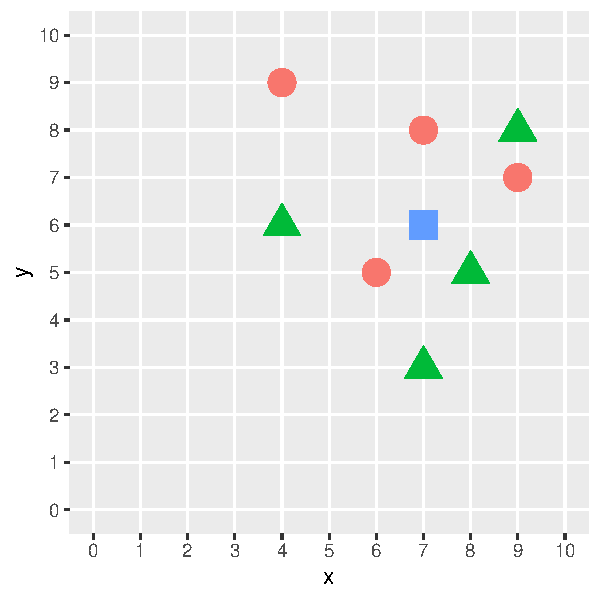
\includegraphics[width=\maxwidth]{figure/unnamed-chunk-18-1} 

}


\end{knitrout}
}
\newpage
\loesung{

\begin{enumerate}
\item[a)] $k = 3$

2 circles and 1 triangle, so our point is also a circle

\begin{knitrout}
\definecolor{shadecolor}{rgb}{0.969, 0.969, 0.969}\color{fgcolor}

{\centering 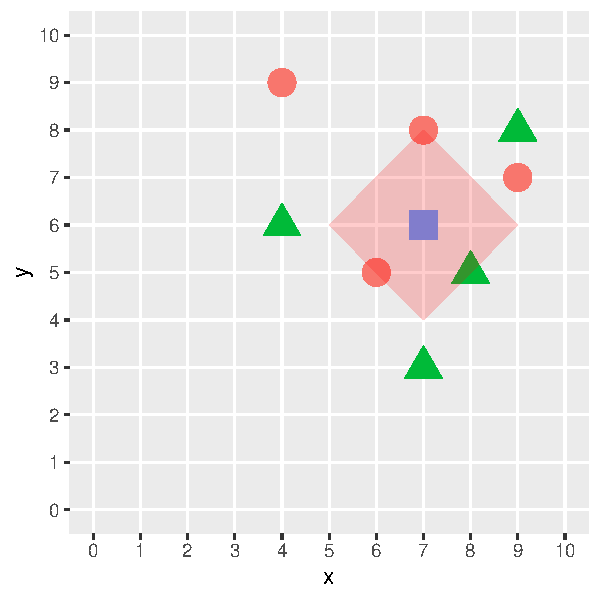
\includegraphics[width=\maxwidth]{figure/unnamed-chunk-19-1} 

}


\end{knitrout}

\item[b)] $k = 5$

3 circles and 3 triangles, we have to specify beforehand what to do in case of a tie

\begin{knitrout}
\definecolor{shadecolor}{rgb}{0.969, 0.969, 0.969}\color{fgcolor}

{\centering 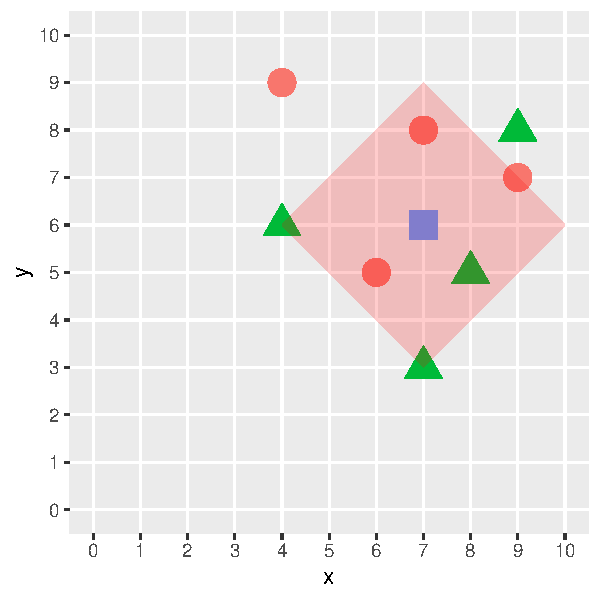
\includegraphics[width=\maxwidth]{figure/unnamed-chunk-20-1} 

}


\end{knitrout}

\item[c)] $k = 7$

3 circles and 4 triangles, so our point is also a triangle

\begin{knitrout}
\definecolor{shadecolor}{rgb}{0.969, 0.969, 0.969}\color{fgcolor}

{\centering 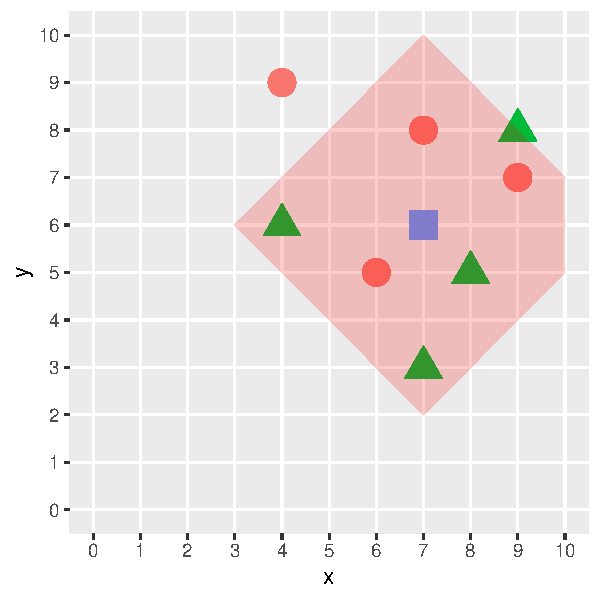
\includegraphics[width=\maxwidth]{figure/unnamed-chunk-21-1} 

}


\end{knitrout}

\end{enumerate}


  
}

\dlz
\aufgabe{$k$-NN from scratch}{

Implement a simple version of a K-nearest-neighbour classifier.

\begin{knitrout}
\definecolor{shadecolor}{rgb}{0.969, 0.969, 0.969}\color{fgcolor}\begin{kframe}
\begin{alltt}
myknn = \hlkwd{function}(target, traindata, testdata, k)
\end{alltt}
\end{kframe}
\end{knitrout}

The function should return a factor of predicted classes from \texttt{testdata}.
\texttt{target} is the name of the target variable in both \texttt{data.frame}s.
Some hints:
\begin{itemize}
\item Your function only needs to work for numeric features.
\item Use the euclidean distance.
\item Do not overengineer your solution. Keep it simple and do not think too much about efficiency.
\end{itemize}

Test your implementation on the \texttt{iris} data set for $k = 1,2,7$.
Split your data set $10$ times in $\frac{2}{3}$ training and $\frac{1}{3}$ test data.
Measure training and test error in each split.
}
\dlz

\loesung{

See \href{https://github.com/compstat-lmu/lecture_i2ml/blob/master/exercises/supervised-classification/sol_knn_from_scratch.R}{R code}
}

\dlz
\aufgabe{QDA from scratch}{

Implement you own version of QDA:\\

\texttt{trainQDA = function(target, data)}\\
\texttt{predictQDA = function(taget,data)}\\

The first function should return the fitted model (use an adequate structure for the model!). The second function should return a factor of classes for \texttt{type = 'class'} and a matrix of predicted probabilities for \texttt{type = 'prob'}. Your method does only need to work for numeric features. Check your implementation on the \texttt{iris} dataset and compare your results of both types with the \texttt{qda()} function from the package \texttt{MASS}.
}
\dlz

\loesung{

See \href{https://github.com/compstat-lmu/lecture_i2ml/blob/master/exercises/supervised-classification/sol_qda_from_scratch.R}{R code}
}

\dlz
\aufgabe{naive Bayes}{

You are given the following table with the target variable \texttt{Banana}:
\begin{center}
\begin{tabular}{ | c | c | c | c | c |}
\hline
ID  &  Color   &  Form    &  Origin    &  Banana ?  \\  \hline
1   &  yellow  &  oblong  &  imported  &  yes       \\
2   &  yellow  &  round   &  domestic  &  no        \\
3   &  yellow  &  oblong  &  imported  &  no        \\
4   &  brown   &  oblong  &  imported  &  yes       \\
5   &  brown   &  round   &  domestic  &  no        \\
6   &  green   &  round   &  imported  &  yes       \\
7   &  green   &  oblong  &  domestic  &  no        \\
8   &  red     &  round   &  imported  &  no        \\
\hline
\end{tabular}
\end{center}

\begin{enumerate}
  \item[a)]
    We want to use a naive Bayes classifier to predict whether a new fruit is a Banana or not. Calculate the posterior probability $\pi(x)$ for a new observation $(\text{yellow}, \text{round}, \text{imported})$. How would you classify the object?

  \item[b)]
    Assume you have an additional feature "Length", which measures the length in cm. Describe in 1-2 sentences how you would handle this numeric feature with Naive Bayes.
\end{enumerate}
}
\dlz
\loesung{

\begin{enumerate}

  \item[a)]

When using the naive Bayes classifier, the features $x := (x_\text{Color},x_\text{Form},x_\text{Origin})$ given the category $y \in \{\text{yes},\text{no}\}$ are assumed to be conditionally independent of each other, s.t.

$$p((x_\text{Color},x_\text{Form},x_\text{Origin})|y = k) = p(x_\text{Color}|y = k)\cdot p(x_\text{Form}|y = k) \cdot p(x_\text{Origin}|y = k).$$

For the posterior probabilities $\pi_k(x)$ it holds that
\begin{align*} \pi_k(x) \propto & \; \underbrace{\pi_k \cdot p(x_\text{Color}|y = k)\cdot p(x_\text{Form}|y = k) \cdot p(x_\text{Origin}|y = k)}_{=: \alpha_k(x)} \\
\iff & \exists c \in \mathbb{R}: \pi_k(x) = c \cdot \alpha_k(x),\end{align*}
where $\pi_k$ is the prior probability of class $k$.
From this and since the posterior probabilities need to sum up to 1, it holds that 
\begin{align*}1 =& \; c \cdot \alpha_\text{yes}(x) +  c \cdot \alpha_\text{no}(x)\\
\iff & c = \frac{1}{\alpha_\text{yes}(x) + \alpha_\text{no}(x)}.
\end{align*}
This means in order to compute $\pi_\text{yes}(x)$ the scores $\alpha_\text{yes}(x)$ and $\alpha_\text{no}(x)$ are needed.\\ Now we want to compute for a new fruit the posterior probability $\hat{\pi}_{yes}((\text{yellow},\text{round},\text{imported}))$. \\
Note that we do not know the \emph{true} prior probability and the \emph{true} conditional densities. Here -since the target and the features are categorical- we can estimate them with the relative frequencies encountered in the data, s.t.
\begin{align*}
\hat{\alpha}_\text{yes}(x) = & \;  \hat{\pi}_{yes} \cdot \hat{p}(\text{yellow}|y = \text{yes})\cdot \hat{p}(\text{round}|y = \text{yes}) \cdot \hat{p}(\text{imported}|y = \text{yes}) \\
= & \; \hat{\P}(y = \text{yes}) \cdot \hat{\P}(x_\text{Color} = \text{yellow}|y = \text{yes})\cdot \hat{\P}(x_\text{Form}=\text{round}|y = \text{yes}) \cdot \hat{\P}(x_\text{Origin}=\text{imported}|y = \text{yes}) \\
= & \; \frac{3}{8} \cdot \frac{1}{3} \cdot \frac{1}{3} \cdot 1 = \frac{1}{24} \approx 0.042, \\
\hat{\alpha}_\text{no}(x) = & \;  \hat{\pi}_{no} \cdot \hat{p}(\text{yellow}|y = \text{no})\cdot \hat{p}(\text{round}|y = \text{no}) \cdot \hat{p}(\text{imported}|y = \text{no}) \\
= & \; \hat{\P}(y = \text{no}) \cdot \hat{\P}(x_\text{Color} = \text{yellow}|y = \text{no})\cdot \hat{\P}(x_\text{Form}=\text{round}|y = \text{no}) \cdot \hat{\P}(x_\text{Origin}=\text{imported}|y = \text{no}) \\
= & \; \frac{5}{8} \cdot \frac{2}{5} \cdot \frac{3}{5} \cdot \frac{2}{5} = \frac{3}{50} = 0.06.
\end{align*}
At this stage we can already see that the predicted label is "no", since $ \hat{\alpha}_\text{no}(x) = 0.06>\frac{1}{24} = 
\hat{\alpha}_\text{yes}(x)$. \\
With this we can calculate the posterior probability
$$\hat{\pi}_\text{yes}(x) = \frac{\hat{\alpha}_\text{yes}(x)}{\hat{\alpha}_\text{yes}(x) + \hat{\alpha}_\text{no}(x)} \approx 0.41.$$


    Corresponding \texttt{R}-Code:

\begin{knitrout}
\definecolor{shadecolor}{rgb}{0.969, 0.969, 0.969}\color{fgcolor}\begin{kframe}
\begin{alltt}
\hlstd{df_banana} \hlkwb{<-} \hlkwd{data.frame}\hlstd{(}
  \hlkwc{Color} \hlstd{=} \hlkwd{as.factor}\hlstd{(}
    \hlkwd{c}\hlstd{(}\hlstr{"yellow"}\hlstd{,} \hlstr{"yellow"}\hlstd{,} \hlstr{"yellow"}\hlstd{,} \hlstr{"brown"}\hlstd{,} \hlstr{"brown"}\hlstd{,} \hlstr{"green"}\hlstd{,} \hlstr{"green"}\hlstd{,} \hlstr{"red"}\hlstd{)),}
  \hlkwc{Form} \hlstd{=} \hlkwd{as.factor}\hlstd{(}
    \hlkwd{c}\hlstd{(}\hlstr{"oblong"}\hlstd{,} \hlstr{"round"}\hlstd{,} \hlstr{"oblong"}\hlstd{,} \hlstr{"oblong"}\hlstd{,} \hlstr{"round"}\hlstd{,} \hlstr{"round"}\hlstd{,} \hlstr{"oblong"}\hlstd{,} \hlstr{"round"}\hlstd{)),}
  \hlkwc{Origin} \hlstd{=} \hlkwd{as.factor}\hlstd{(}
    \hlkwd{c}\hlstd{(}\hlstr{"imported"}\hlstd{,} \hlstr{"domestic"}\hlstd{,} \hlstr{"imported"}\hlstd{,} \hlstr{"imported"}\hlstd{,} \hlstr{"domestic"}\hlstd{,} \hlstr{"imported"}\hlstd{,}
    \hlstr{"domestic"}\hlstd{,} \hlstr{"imported"}\hlstd{)),}
  \hlkwc{Banana} \hlstd{=} \hlkwd{as.factor}\hlstd{(}\hlkwd{c}\hlstd{(}\hlstr{"yes"}\hlstd{,} \hlstr{"no"}\hlstd{,} \hlstr{"no"}\hlstd{,} \hlstr{"yes"}\hlstd{,} \hlstr{"no"}\hlstd{,} \hlstr{"yes"}\hlstd{,} \hlstr{"no"}\hlstd{,} \hlstr{"no"}\hlstd{))}
\hlstd{)}

\hlstd{new_fruit} \hlkwb{<-} \hlkwd{data.frame}\hlstd{(}\hlkwc{Color} \hlstd{=} \hlstr{"yellow"}\hlstd{,} \hlkwc{Form} \hlstd{=} \hlstr{"round"}\hlstd{,} \hlkwc{Origin} \hlstd{=} \hlstr{"imported"}\hlstd{,} \hlkwc{Banana} \hlstd{=} \hlnum{NA}\hlstd{)}
\hlstd{df_banana} \hlkwb{<-} \hlkwd{rbind}\hlstd{(df_banana, new_fruit)}

\hlkwd{library}\hlstd{(mlr3)}
\hlkwd{library}\hlstd{(mlr3learners)}

\hlstd{nb_learner} \hlkwb{<-} \hlkwd{lrn}\hlstd{(}\hlstr{"classif.naive_bayes"}\hlstd{,}
                  \hlkwc{predict_type} \hlstd{=} \hlstr{"prob"}\hlstd{)}

\hlstd{banana_task} \hlkwb{<-} \hlstd{TaskClassif}\hlopt{$}\hlkwd{new}\hlstd{(}
  \hlkwc{id} \hlstd{=} \hlstr{"banana"}\hlstd{,}
  \hlkwc{backend} \hlstd{= df_banana,}
  \hlkwc{target} \hlstd{=} \hlstr{"Banana"}
\hlstd{)}

\hlstd{nb_learner}\hlopt{$}\hlkwd{train}\hlstd{(banana_task,} \hlkwc{row_ids}\hlstd{=}\hlnum{1}\hlopt{:}\hlnum{8}\hlstd{)}

\hlstd{nb_learner}\hlopt{$}\hlkwd{predict}\hlstd{(banana_task,} \hlkwc{row_ids} \hlstd{=} \hlnum{9}\hlstd{)}
\end{alltt}
\begin{verbatim}
## <PredictionClassif> for 1 observations:
##  row_ids truth response   prob.no  prob.yes
##        9  <NA>       no 0.5901639 0.4098361
\end{verbatim}
\end{kframe}
\end{knitrout}

  \item[b)]
    For the distribution of a numerical feature given the the category we need to specify a probability distribution with continuous support.
    For example, for the information $x_\text{Length}$ we could assume that $p(x_\text{Length} | y = \text{yes}) \sim \mathcal{N}(\mu_\text{yes},\sigma^2_\text{yes})$ and $p(x_\text{Length} | y = \text{no}) \sim \mathcal{N}(\mu_\text{no},\sigma^2_\text{no})$. (To estimate these normal distributions one would need to estimate their parameters $\mu_\text{yes},\mu_\text{no},\sigma^2_\text{yes},\sigma^2_\text{no}$ on the data respectively)
\end{enumerate}
}

\dlz
\aufgabe{classifying \texttt{ionosphere}}{

Take a look at the Ionosphere dataset from the \texttt{mlbench} package and descripe the dataset shortly. You don't have to summarize all its statistical properties but rather what kind of classification problem it is. Which classifiers from the lecture seem to be applicable for the dataset? Descripe independently of your code how you proceeded to in your analysis and what your results are.\\
\textbf{Note:} You don't have to check every single classifier in every configuration, more importantly is a smart approach with moderate effort. Use \texttt{mlr} for your analysis.
}
\dlz
\loesung{

No model solution
}

% ------------------------------------------------------------------------------
% PAST EXAMS
% ------------------------------------------------------------------------------

\dlz
\exexams
\lz

\aufgabeexam{WS2020/21}{main}{1}{

\begin{knitrout}
\definecolor{shadecolor}{rgb}{0.969, 0.969, 0.969}\color{fgcolor}

{\centering 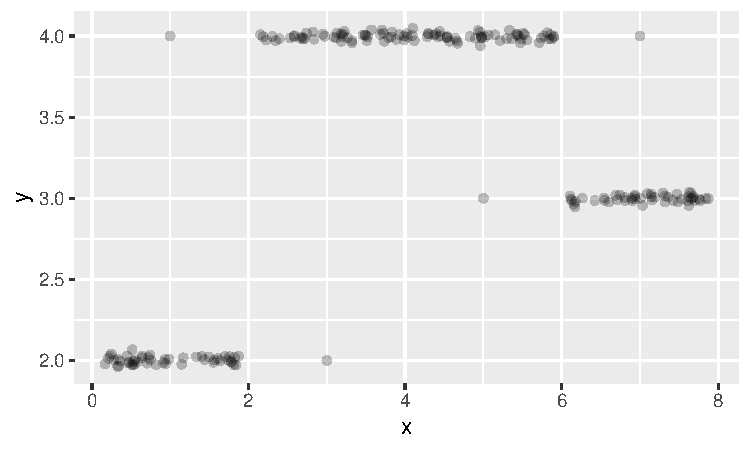
\includegraphics[width=\maxwidth]{figure/unnamed-chunk-15-1} 

}


\end{knitrout}

The above plot shows $\D = \Dset $, a data set with %$n$ observations
%data $\xv = (x^{(1)}, \dots, x^{(n)})^\top$ and $\ydat = \yvec$ for 
$n$ = 200 observations of a continuous target variable $y$ and a continuous, 
1-dimensional feature variable $\xv$. In the following, we aim at predicting 
$y$ with a machine learning model that takes $\xv$ as input.

\begin{enumerate}
  \item Since the data seem to fall in 3 quite well-separable classes, we now 
  want to apply a classification model instead of the regression model in a). 
  To prepare the data for classification, we categorize the target variable $y$ 
  in 3 classes and call the transformed target variable $z$, as follows:
  \[
    z^{(i)} = \left\{\begin{array}{lr}
        1, \text{ if }&  -\infty < \yi \leq 2.5 \\
        2, \text{ if }&  2.5\ < \yi \leq 3.5 \\
        3, \text{ if }&  3.5 < \yi < \infty
        \end{array} \right\}
  \]
  Now we can apply quadratic discriminant analysis (QDA):
  \begin{enumerate}
    \item[(i)] Estimate the class means $\mu_k = \E(\xv|z = k)$ for each of the 
    three classes $k \in \{1, 2, 3\}$ visually from the plot. Do not 
    overcomplicate this, a rough estimate is sufficient here.
    \item[(ii)] Make a hand-drawn plot that visualizes the different estimated 
    densities per class.
    \item[(iii)] How would your drawing from (ii) change if we used linear 
    discriminant analysis (LDA) instead of QDA? Explain your answer.
    \item[(iv)] Why is QDA for this data preferable over LDA?
  \end{enumerate}  
  \item Given are two new observations $\xv_{*1} = -10$ and $\xv_{*2} = 7$. 
  State the prediction for each of the two models 
  \begin{enumerate}
    \item[(i)] regression tree
    \item[(ii)] QDA
  \end{enumerate}
  and explain how you derived the predictions.
  \item Discuss in 1-2 sentences which of the 2 models (regression tree, QDA) 
  you would prefer for modeling the data and explain your decision.
\end{enumerate}

\dlz
\loesung{

\begin{enumerate}
  \item \phantom{foo}
  \begin{enumerate}
    \item[(i)] $\mu_1 = 1$, $\mu_2 = 7$, $\mu_3 = 4$
    \item[(ii)] 
\begin{knitrout}
\definecolor{shadecolor}{rgb}{0.969, 0.969, 0.969}\color{fgcolor}
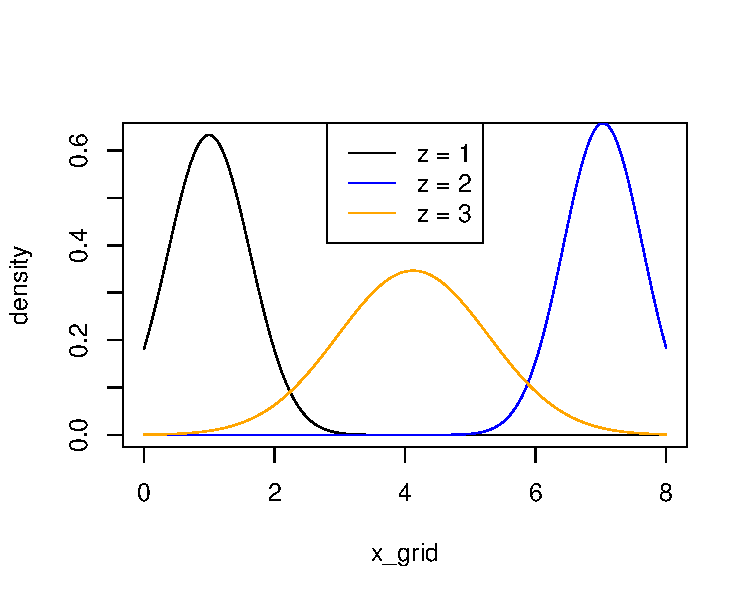
\includegraphics[width=\maxwidth]{figure/unnamed-chunk-16-1} 
\end{knitrout}
    \item[(iii)] Variances would be all equal. Assumption of LDA is equal 
    variances, i.e., estimatated models will always have equal variances, no 
    matter if this fits the data or not
    \item[(iv)] Variances seem not to be equal, this is only captured in QDA
  \end{enumerate}  
  \item \phantom{foo}
  \begin{enumerate}
    \item[(i)] $\hat{y}_{*1} = 2$, $\hat{y}_{*2} = 3$, 
    \item[(ii)] $\hat{z}_{*1} = 3$, since the variance of class 3 is higher, 
    the density will overshoot the density of class 1. 
    $\hat{z}_{*2} = 2$, obviously highest posterior here.
  \end{enumerate}
  \item E.g., 
  \begin{itemize}
    \item CART better than LM because I do not have to specify those indicator 
    functions manually and estimate the split points manually, CART does this 
    data driven
    \item For QDA we have to throw away information of y, this favors CART
    \item QDA predicts the middle class (3) for very extreme observations, this 
    does not seem right. However, we do not know how data behave outside the 
    bounds of x.
    \item QDA assumes gaussian distributions which is clearly not the case.
  \end{itemize}
\end{enumerate}

}

% ------------------------------------------------------------------------------

\dlz
\aufgabeexam{WS2020/21}{main}{4}{

The table below shows $\D = \Dset $, a data set with 
$n$ = 8 observations of a binary target variable $y$ containing the information 
if the object is a \texttt{Banana} or not and a 4-dimensional feature vector 
$\xv$, containing \texttt{Color}, \texttt{Form}, \texttt{Origin} (categorical 
features) and \texttt{Length} (continuous feature) of the object. In the 
following, we aim at predicting \texttt{Banana} with a machine learning model 
that takes $\xv$ as input.

\begin{tabular}{ | c | c | c | c | c | c |}
\hline
ID  &  Color   &  Form    &  Origin    & Length [cm]  &  Banana  \\  \hline
1   &  yellow  &  oblong  &  imported  & 15           &  yes      \\
2   &  yellow  &  round   &  domestic  & 5            &  no       \\
3   &  yellow  &  oblong  &  imported  & 10           &  no       \\
4   &  brown   &  oblong  &  imported  & 17           &  yes      \\
5   &  brown   &  round   &  domestic  & 16           &  no        \\
6   &  green   &  round   &  imported  & 13           &  yes       \\
7   &  green   &  oblong  &  domestic  & 25           &  no       \\
8   &  red     &  round   &  imported  & 7            &  no        \\
\hline
\end{tabular}

We want to use a naive Bayes classifier to predict the label of a new 
observation. 

\begin{enumerate}
  \item Calculate the posterior probability $\pi(\xv_*) = \P(y = \text{yes} | 
  \xv_*)$ for a new observation \ $\xv_* = (\text{green}, \text{oblong}, 
  \text{imported}, 14)^\top$. Explain every step thoroughly. (Hint: At some 
  point you will have to compute values of Gaussian densities - use R for this
  step.)
  \item How would you classify the new observation? Explain your answer.
\end{enumerate}

}

\dlz
\loesung{

\begin{enumerate}

  \item The features $\xv := (x_\text{Color},x_\text{Form},x_\text{Origin},
  x_\text{Length})$ given the category $y \in \{\text{yes},\text{no}\}$ are
  assumed to be conditionally independent of each other (since we are using
  Naive Bayes), s.t.

  $$p(\xv|y = k) = p(x_\text{Color}|y = k)\cdot p(x_\text{Form}|y = k) \cdot
  p(x_\text{Origin}|y = k) \cdot p(x_\text{Length}|y = k).$$

  For the posterior probabilities $\pi_k(\xv) = \P(y = k | \xv)$ it holds with
  Bayes' Theorem:
  \begin{align*}
  \pi_k(\xv)  \propto & \; \underbrace{\pi_k \cdot p(\xv|y = k)
  }_{=: \alpha_k(\xv)} \\
  \iff & \exists c \in \mathbb{R}: \pi_k(\xv) = c \cdot \alpha_k(\xv),
  \end{align*}

  where $\pi_k = \P(y = k)$ is the prior probability of class $k$.

  From this and since the posterior probabilities need to sum up to 1, it holds
  that
  \begin{align*}1 =& \; c \cdot \alpha_\text{yes}(\xv) +  c \cdot
  \alpha_\text{no}(\xv) \\
  \iff & c = \frac{1}{\alpha_\text{yes}(\xv) + \alpha_\text{no}(\xv)}.
  \end{align*}

  This means, the scores $\alpha_\text{yes}(x)$ and $\alpha_\text{no}(x)$ are
  needed to compute  $$\pi_\text{yes}(\xv) = \frac{\alpha_\text{yes}(\xv)}{
  \alpha_\text{yes}(\xv) + \alpha_\text{no}(\xv)}. $$

  For the new observation $\xv_*$ we have to estimate the respective
  probabilities and densities. For the categorical features, we can simply
  compute relative frequencies. For the continuous features \texttt{Length} we
  have to estimate the densities per class and evaluate those at the value $14$.
  Doing this with R we end up with:

\begin{knitrout}
\definecolor{shadecolor}{rgb}{0.969, 0.969, 0.969}\color{fgcolor}\begin{kframe}
\begin{verbatim}
## [1] 0.1760327
## [1] 0.04863352
\end{verbatim}
\end{kframe}
\end{knitrout}

  \begin{center}
  \begin{tabular}{ | c | c | c | c | c | c |}
  \hline
  k     &  $\hat{\pi}_k$   &  $\hat{p}(\text{green}|y = k)$    &  
  $\hat{p}(\text{oblong}|y = k)$    & $\hat{p}(\text{imported}|y = k)$    & 
  $\hat{p}(\text{14}|y = k)$   \\  \hline
  yes   &  3/8  &  1/3    &  2/3  & 3/3     &  0.176 \\
  no    &  5/8  &  1/5    &  2/5  & 2/5     &  0.049 \\
  \hline
  \end{tabular}
  \end{center}

  \begin{align*}
  \hat{\alpha}_\text{yes}(x) = & \;  \hat{\pi}_{yes} \cdot \hat{p}(
  \text{green}|y = \text{yes})\cdot \hat{p}(\text{oblong}|y = \text{yes}) \cdot 
  \hat{p}(\text{imported}|y = \text{yes}) \cdot \hat{p}(14|y = \text{yes}) \\
  = & \; \frac{3}{8} \cdot \frac{1}{3} \cdot \frac{2}{3} \cdot 1 \cdot 0.176  
  \approx 0.0147, \\
  \hat{\alpha}_\text{no}(x) = & \;  
  \hat{\pi}_{no} \cdot \hat{p}(\text{green}|y = \text{no})\cdot 
  \hat{p}(\text{oblong}|y = \text{no}) \cdot \hat{p}(\text{imported}|y = 
  \text{no}) \cdot \hat{p}(14|y = \text{no}) \\
  = & \; \frac{5}{8} \cdot \frac{1}{5} \cdot \frac{2}{5} \cdot \frac{2}{5} 
  \cdot 0.049  \approx 0.00098.
  \end{align*}
  
  With this we can calculate the posterior probability
  $$\hat{\pi}_\text{yes}(x) = \frac{\hat{\alpha}_\text{yes}(x)}{
  \hat{\alpha}_\text{yes}(x) + \hat{\alpha}_\text{no}(x)} \approx 0.937.$$
  
  \item Classification as yes = \texttt{banana}. We have to define a threshold, 
  observations with a posterior probability equal or above the threshold are 
  hard labeled as yes, others as no. The optimal threshold has to be chosen, 
  e.g., inspecting ROC measures. With default 0.5 we end up with the above 
  classification.

\end{enumerate}
}

% ------------------------------------------------------------------------------
% INSPO
% ------------------------------------------------------------------------------

\dlz
\exinspo
\end{document}
